% $HeadURL$

%%%%%%%%%%%%%%%%%%%%%%%%%%%%%%%%%%%%%%%%%%%%%%%%%%%%%%%%%%%%%%%%%%%%%%
%%                     Trigger
%%%%%%%%%%%%%%%%%%%%%%%%%%%%%%%%%%%%%%%%%%%%%%%%%%%%%%%%%%%%%%%%%%%%%%

\subsection{Glyph: \glyph{Trigger}}\label{sec:trigger}

A trigger effect, or absolute stimulation, is a stimulation that is necessary for a process to take place. A process modulated by a trigger can only occur when this trigger is active.

\begin{glyphDescription}
 \glyphSboTerm SBO:0000171 ! necessary stimulation.
 \glyphOrigin Any \glyph{EPN} (\sect{EPNs}) or any \glyph{logical operator} (\sect{logic}).
 \glyphTarget Any \glyph{process node} (\sect{PNs}).
 \glyphNode The target extremity of a \glyph{trigger} carries an open arrow (to remind that it is a \glyph{stimulation}) coming after a larger vertical bar.
 \end{glyphDescription}

\begin{figure}[H]
  \centering
  
\includegraphics[scale = 0.5]{images/trigger}
  \caption{The \PD glyph for \glyph{trigger}.}
  \label{fig:trigger}
\end{figure}

The example in \fig{trigger-gene} below describes the transcription of a gene~X, that is the creation of a messenger RNA~X triggered by the gene~X.  The creation of the protein~X is then triggered by the mRNA~X.  (Note that the same example could be represented using the gene as reactant and product, although it is semantically different.)

\begin{figure}[H]
  \centering
  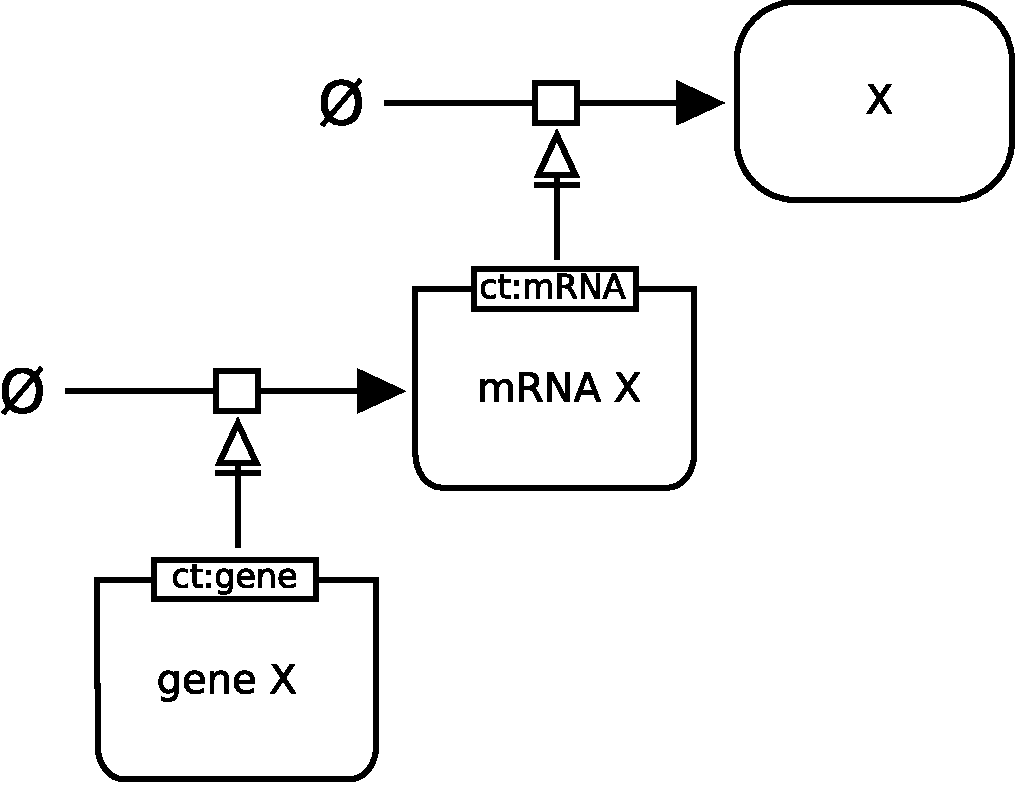
\includegraphics[scale = 0.5]{examples/trigger-genetic}
  \caption{The creation of a messenger RNA~X triggered by the gene~X.}
  \label{fig:trigger-gene}
\end{figure}


The example in \fig{trigger-calcium} below describes the transport of calcium ions out of the endoplasmic reticulum. Without IP3 receptor, there is not calcium flux, therefore, one cannot use a \glyph{stimulation}. The trigger instead represents this absolute stimulation.

\begin{figure}[H]
  \centering
  \includegraphics[scale = 0.5]{examples/trigger-transport}
  \caption{The transport of calcium ions out of the endoplasmic reticulum.}
  \label{fig:trigger-calcium}
\end{figure}



% The following is for [X]Emacs users.  Please leave in place.
% Local Variables:
% TeX-master: "../sbgn_PD-level1"
% End:
